% !TEX program = lualatex
% Μεταγλώττιση:  lualatex Διάλεξη2_γραφήματα.tex   (δύο φορές, για τα περιεχόμενα)
\documentclass[11pt,a4paper]{article}

% ------------------------------------------------------------------ προοίμιο
\usepackage[a4paper,margin=2.3cm,headheight=14pt]{geometry}
\usepackage{amsmath}
\usepackage{fontspec}
\usepackage{unicode-math}
\usepackage{tikz}                   % πριν από το polyglossia: αλλιώς το arrows.meta δεν φορτώνει
\usetikzlibrary{arrows.meta}
\usepackage{polyglossia}
\setmainlanguage{greek}
\setotherlanguage{english}
% Οι γραμματοσειρές φορτώνονται με όνομα αρχείου (υπάρχουν στο TeX Live).
\newcommand{\serif}{LibertinusSerif}
\setmainfont{\serif}[Ligatures=TeX, Extension=.otf, UprightFont=*-Regular, BoldFont=*-Bold,
  ItalicFont=*-Italic, BoldItalicFont=*-BoldItalic]
\setsansfont{LibertinusSans}[Ligatures=TeX, Extension=.otf, UprightFont=*-Regular, BoldFont=*-Bold,
  ItalicFont=*-Italic]
\setmonofont{DejaVuSansMono}[Extension=.ttf, UprightFont=*, BoldFont=*-Bold,
  ItalicFont=*-Oblique, BoldItalicFont=*-BoldOblique, Scale=0.84, Ligatures=ResetAll]
\setmathfont{LibertinusMath-Regular.otf}
\newfontfamily\greekfont{\serif}[Ligatures=TeX, Extension=.otf, UprightFont=*-Regular, BoldFont=*-Bold,
  ItalicFont=*-Italic, BoldItalicFont=*-BoldItalic]
\newfontfamily\greekfontsf{LibertinusSans}[Ligatures=TeX, Extension=.otf, UprightFont=*-Regular,
  BoldFont=*-Bold, ItalicFont=*-Italic]
\newfontfamily\greekfonttt{DejaVuSansMono}[Extension=.ttf, UprightFont=*, BoldFont=*-Bold,
  ItalicFont=*-Oblique, BoldItalicFont=*-BoldOblique, Scale=0.84, Ligatures=ResetAll]

\usepackage{xcolor}
\usepackage{booktabs}
\usepackage{tabularx}
\usepackage{array}
\newcolumntype{Y}{>{\raggedright\arraybackslash}X}
\usepackage{enumitem}
\usepackage[most]{tcolorbox}
\usepackage{piton}
\usepackage{fvextra}
\usepackage{fancyhdr}
\usepackage{titlesec}
\usepackage[hidelinks]{hyperref}

\definecolor{codebg}{gray}{0.965}
\definecolor{kw}{RGB}{0,70,150}
\definecolor{cm}{RGB}{40,110,40}
\definecolor{st}{RGB}{160,40,40}
\definecolor{accent}{RGB}{0,70,150}
\definecolor{gold}{RGB}{255,215,0}
\definecolor{edgecol}{RGB}{30,60,200}

% Κώδικας Python: πακέτο piton (χρειάζεται LuaLaTeX). Έξοδοι προγραμμάτων: fvextra.
\PitonOptions{background-color=codebg, splittable=3, break-lines, left-margin=auto}
\SetPitonStyle{Comment = \color{cm}, String = \color{st}, String.Doc = \color{cm},
  Interpol.Inside = \color{black}, Keyword = \color{kw}\bfseries,
  Keyword.Constant = \color{kw}\bfseries, Operator.Word = \color{kw}\bfseries,
  Number = \color{black}, Name.Builtin = \color{kw}, Name.Function = \bfseries,
  Name.Class = \bfseries, Name.Namespace = \color{black}, Exception = \color{st}\bfseries}
\AddToHook{env/Piton/begin}{\small}
\newcommand{\pyfile}[1]{{\small\PitonInputFile{#1}}}
\DefineVerbatimEnvironment{output}{Verbatim}{frame=single, rulecolor=\color{gray!40},
  fontsize=\small, xleftmargin=10pt, breaklines}

\newcommand{\code}[1]{\texttt{#1}}
\newcommand{\prog}[1]{\textsf{\bfseries #1}}
% Επιτρέπουμε αλλαγή γραμμής μετά από κάθε _ (μεγάλα ονόματα αρχείων).
\renewcommand{\_}{\textunderscore\allowbreak}

\newtcolorbox{note}[1][Προσοχή]{colback=accent!4, colframe=accent!60, fonttitle=\bfseries\sffamily,
  title=#1, boxrule=0.6pt, arc=2pt, left=6pt, right=6pt, top=4pt, bottom=4pt}

% Σχήματα γραφημάτων: οι κορυφές πάνω σε κύκλο, όπως στη draw των προγραμμάτων
% (η κορυφή v στη γωνία 360·v/n μοίρες: η 0 δεξιά, οι επόμενες αριστερόστροφα).
\tikzset{
  vertex/.style={circle, fill=gold, draw=gold!60!black, minimum size=1.35cm, inner sep=0pt,
    font=\footnotesize\sffamily},
  small vertex/.style={circle, fill=gold, draw=gold!60!black, minimum size=0.6cm, inner sep=0pt,
    font=\small\sffamily},
  edge/.style={edgecol, thick},
  arc/.style={edgecol, thick, -{Stealth[length=2.6mm]}, bend left=12, shorten >=1pt},
}

\titleformat{\section}{\Large\sffamily\bfseries\color{accent}}{\thesection}{0.6em}{}
\titleformat{\subsection}{\large\sffamily\bfseries}{\thesubsection}{0.6em}{}
\setlist{itemsep=2pt, topsep=4pt}
\renewcommand{\arraystretch}{1.25}
\setlength{\emergencystretch}{3em}

\pagestyle{fancy}
\fancyhf{}
\lhead{\small\sffamily Πληροφορική Ι}
\rhead{\small\sffamily Διάλεξη 2 — Γραφήματα}
\cfoot{\small\thepage}

\begin{document}

% ------------------------------------------------------------------ τίτλος
\begin{center}
  {\sffamily\small ΠΛΗΡΟΦΟΡΙΚΗ Ι \quad·\quad 2026–2027}\\[6pt]
  {\sffamily\bfseries\huge\color{accent} Διάλεξη 2}\\[4pt]
  {\sffamily\Large Γραφήματα με λίστες}
\end{center}
\vspace{4pt}

\noindent\textbf{Στόχος.} Να αποθηκεύσουμε ένα \textbf{γράφημα} με λίστες (λίστα ακμών, λίστες
γειτνίασης), να απαντάμε ερωτήσεις πάνω του (βαθμοί, γείτονες, κοινοί γνωστοί), να το ζωγραφίζουμε
με το \code{matplotlib}, και να γράψουμε τις πρώτες συναρτήσεις που φτιάχνουν και μετασχηματίζουν
γραφήματα.

\begin{center}
\small
\begin{tabularx}{\linewidth}{@{}c >{\raggedright\arraybackslash}p{0.36\linewidth} Y@{}}
\toprule
& \textbf{Πρόγραμμα} & \textbf{Τι δείχνει} \\
\midrule
1 & \prog{1\_μη\_κατευθυνόμενα\_γραφήματα.py} & λίστα ακμών, λίστες γειτνίασης, βαθμοί, κοινοί
  γνωστοί, σχέδιο με γραμμές \\
2 & \prog{2\_κατευθυνόμενα\_γραφήματα.py} & βέλη, εξερχόμενοι και εισερχόμενοι γείτονες, έξω- και
  έσω-βαθμοί, αμοιβαίες ακμές, σχέδιο με βέλη \\
3 & \prog{3\_αντίστροφο\_γράφημα.py} & συναρτήσεις πάνω σε γραφήματα: τυχαίο γράφημα, αντίστροφο
  γράφημα, δύο σχήματα δίπλα-δίπλα \\
\bottomrule
\end{tabularx}
\end{center}

\tableofcontents

% =========================================================================
\section{Ορισμοί}

Ένα \textbf{γράφημα} $G = (V, E)$ αποτελείται από ένα σύνολο \textbf{κορυφών} $V$ και ένα σύνολο
\textbf{ακμών} $E$. Κάθε ακμή είναι ένα ζεύγος κορυφών. Παραδείγματα: σε ένα κοινωνικό δίκτυο οι
κορυφές είναι άνθρωποι και οι ακμές γνωριμίες. Σε έναν χάρτη οι κορυφές είναι πόλεις και οι ακμές
δρόμοι. Στον παγκόσμιο ιστό οι κορυφές είναι σελίδες και οι ακμές σύνδεσμοι.

\begin{itemize}
  \item \textbf{Μη κατευθυνόμενο} γράφημα: η ακμή $\{u, v\}$ δεν έχει φορά. Αν η $u$ γνωρίζει τη $v$,
        τότε και η $v$ γνωρίζει τη $u$.
  \item \textbf{Κατευθυνόμενο} γράφημα: η ακμή $(u, v)$ είναι ένα \textbf{βέλος} $u \to v$
        (π.χ.\ «ο $u$ ακολουθεί τον $v$»). Αυτό δεν σημαίνει ότι υπάρχει και το $v \to u$.
  \item \textbf{Γείτονες} της $v$: οι κορυφές που συνδέονται με την $v$ με ακμή.
  \item \textbf{Βαθμός} $\deg(v)$: το πλήθος των γειτόνων της $v$. Σε κατευθυνόμενο γράφημα
        ξεχωρίζουμε τον \textbf{έξω-βαθμό} (πόσα βέλη φεύγουν από τη $v$) και τον \textbf{έσω-βαθμό}
        (πόσα βέλη φτάνουν στη $v$).
\end{itemize}

\begin{note}[Βασική ιδέα]
Αριθμούμε τις κορυφές $0, 1, \dots, n-1$, ώστε να είναι \textbf{δείκτες σε λίστες}. Αν οι κορυφές
έχουν ονόματα, τα κρατάμε σε μια λίστα \code{names} και η κορυφή \code{v} έχει όνομα \code{names[v]}.
\end{note}

% =========================================================================
\section{Μη κατευθυνόμενα γραφήματα}
\noindent Πρόγραμμα: \prog{1\_μη\_κατευθυνόμενα\_γραφήματα.py}. Έξι φίλοι και επτά γνωριμίες
(Σχήμα~\ref{fig:undirected}).

\begin{figure}[h]
  \centering
  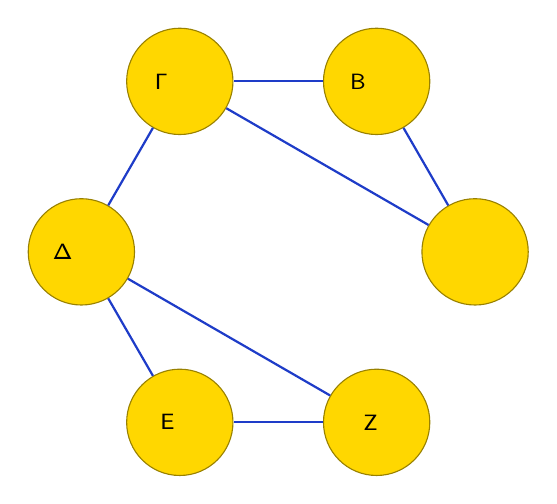
\begin{tikzpicture}
    \foreach \v/\name in {0/Άννα, 1/Βασίλης, 2/Γιώργος, 3/Δήμητρα, 4/Ελένη, 5/Ζωή}
      \node[vertex] (\v) at ({60*\v}:2.5cm) {\name};
    \foreach \u/\v in {0/1, 0/2, 1/2, 2/3, 3/4, 3/5, 4/5}
      \draw[edge] (\u) -- (\v);
  \end{tikzpicture}
  \caption{Το γράφημα του \prog{1\_μη\_κατευθυνόμενα\_γραφήματα.py}, όπως το ζωγραφίζει η
    \code{draw}.}
  \label{fig:undirected}
\end{figure}

\subsection{Λίστα ακμών}
\begin{Piton}
names = ['Άννα', 'Βασίλης', 'Γιώργος', 'Δήμητρα', 'Ελένη', 'Ζωή']   # names[v]
n = len(names)
edges = [[0, 1], [0, 2], [1, 2], [2, 3], [3, 4], [3, 5], [4, 5]]
\end{Piton}

Κάθε ακμή είναι μια λίστα με 2 στοιχεία. Θα μπορούσε να είναι και πλειάδα \code{(0, 1)} (Διάλεξη 1,
§7). Στο μη κατευθυνόμενο γράφημα τα \code{[0, 1]} και \code{[1, 0]} είναι η ίδια ακμή, οπότε τη
γράφουμε μία φορά. Το πλήθος των ακμών είναι \code{len(edges)}.

\subsection{Λίστες γειτνίασης}
Η λίστα ακμών δεν απαντά εύκολα στην ερώτηση «ποιοι είναι οι γείτονες της \code{v};»: πρέπει να
σαρώσουμε όλες τις ακμές. Γι' αυτό φτιάχνουμε \textbf{μία λίστα για κάθε κορυφή}: \code{adj[v]} είναι
η λίστα με τους γείτονες της \code{v}. Η \code{adj} είναι μια λίστα από λίστες.

\begin{Piton}
adj = [[] for i in range(n)]
for u, v in edges:
    adj[u].append(v)
    adj[v].append(u)        # μη κατευθυνόμενο: η ακμή μπαίνει και στις δύο μεριές
# adj = [[1, 2], [0, 2], [0, 1, 3], [2, 4, 5], [3, 5], [3, 4]]
\end{Piton}

Το \code{for u, v in edges} «ξεπακετάρει» κάθε ακμή: για την \code{[0, 1]} είναι \code{u = 0} και
\code{v = 1}. Επειδή η ακμή δεν έχει φορά, η \code{v} μπαίνει στους γείτονες της \code{u}
\textbf{και} η \code{u} στους γείτονες της \code{v}.

\begin{note}
Το \code{[[]] * n} φτιάχνει μια λίστα με την \textbf{ίδια} κενή λίστα \code{n} φορές (Διάλεξη 1,
§6). Ένα \code{append} σε μία κορυφή θα εμφανιζόταν σε όλες. Η \code{[[] for i in range(n)]}
φτιάχνει \code{n} \textbf{διαφορετικές} κενές λίστες.
\end{note}

\begin{note}[f-strings]
Το πρόγραμμα τυπώνει τις λίστες γειτνίασης με ένα \textbf{f-string}:
\begin{Piton}
print(f'{v} {names[v]:8} -> {adj[v]}   {[names[u] for u in adj[v]]}')
\end{Piton}
Το \code{f} πριν από τα εισαγωγικά σημαίνει ότι ό,τι είναι μέσα σε άγκιστρα \code{\{ \}} είναι
\textbf{έκφραση} Python: υπολογίζεται και η τιμή της μπαίνει μέσα στο κείμενο. Το \code{:8} στο
\code{\{names[v]:8\}} συμπληρώνει το όνομα με κενά ώς τους 8 χαρακτήρες, ώστε οι στήλες να
στοιχίζονται. Η τελευταία έκφραση είναι μια list comprehension που μετατρέπει τους αριθμούς των
γειτόνων σε ονόματα.
\end{note}

\subsection{Ερωτήσεις πάνω στο γράφημα}
Με τις λίστες γειτνίασης οι περισσότερες ερωτήσεις γίνονται μία γραμμή:

\begin{center}
\begin{tabularx}{\linewidth}{@{}l Y@{}}
\toprule
\textbf{Ερώτηση} & \textbf{Κώδικας} \\
\midrule
βαθμός κάθε κορυφής & \code{deg = [len(adj[v]) for v in range(n)]} \\
ο πιο «κοινωνικός» & \code{names[deg.index(max(deg))]} \\
γνωρίζονται οι \code{u} και \code{v}; & \code{v in adj[u]} \\
κοινοί γνωστοί των \code{u} και \code{v} & \code{[w for w in adj[u] if w in adj[v]]} \\
\bottomrule
\end{tabularx}
\end{center}

\textbf{Λήμμα της χειραψίας:} $\sum_v \deg(v) = 2|E|$, γιατί κάθε ακμή μπαίνει σε \textbf{δύο} λίστες
γειτνίασης. Εδώ $14 = 2 \cdot 7$, και το πρόγραμμα το ελέγχει.

Ο Γιώργος και η Δήμητρα έχουν και οι δύο βαθμό 3. Η \code{deg.index(max(deg))} επιστρέφει την
\textbf{πρώτη} θέση όπου εμφανίζεται το μέγιστο, γι' αυτό τυπώνεται μόνο ο Γιώργος.

\begin{output}
Κορυφές: 6   Ακμές: 7

0 Άννα     -> [1, 2]   ['Βασίλης', 'Γιώργος']
1 Βασίλης  -> [0, 2]   ['Άννα', 'Γιώργος']
2 Γιώργος  -> [0, 1, 3]   ['Άννα', 'Βασίλης', 'Δήμητρα']
3 Δήμητρα  -> [2, 4, 5]   ['Γιώργος', 'Ελένη', 'Ζωή']
4 Ελένη    -> [3, 5]   ['Δήμητρα', 'Ζωή']
5 Ζωή      -> [3, 4]   ['Δήμητρα', 'Ελένη']

Βαθμοί: [2, 2, 3, 3, 2, 2]
Άθροισμα βαθμών = 14 = 2 x πλήθος ακμών = 14
Ο πιο "κοινωνικός": Γιώργος
Γνωρίζονται 0 και 1; True
Γνωρίζονται 0 και 5; False
Κοινοί γνωστοί των Άννα και Δήμητρα: ['Γιώργος']
\end{output}

\subsection{Σχέδιο με το matplotlib}
Η συνάρτηση \code{draw(names, edges)} τοποθετεί την κορυφή \code{v} στο σημείο
$\bigl(\cos(2\pi v/n),\, \sin(2\pi v/n)\bigr)$ του μοναδιαίου κύκλου. Έτσι οι $n$ κορυφές ισαπέχουν:
η 0 είναι δεξιά και οι επόμενες ακολουθούν αριστερόστροφα. Οι συντεταγμένες μπαίνουν σε δύο λίστες,
\code{px} και \code{py}.

\begin{itemize}
  \item \code{plt.plot([px[u], px[v]], [py[u], py[v]], 'b')}: ευθύγραμμο τμήμα από τη \code{u} στη
        \code{v}. Η πρώτη λίστα έχει τα $x$ και η δεύτερη τα $y$ των άκρων.
  \item \code{plt.plot(px, py, 'o', ms=25, color='gold')}: όλες οι κορυφές μαζί, ως μεγάλοι κίτρινοι
        κύκλοι. Ζωγραφίζονται \textbf{μετά} τις ακμές, ώστε να σκεπάζουν τις άκρες τους.
  \item \code{plt.text(px[v], py[v], names[v], ha='center', va='center')}: το όνομα στο κέντρο του
        κύκλου.
  \item \code{plt.axis('equal')}: ίδια κλίμακα στους δύο άξονες, αλλιώς ο κύκλος γίνεται έλλειψη.
        \code{plt.axis('off')}: κρύβει τους άξονες.
\end{itemize}

Η \code{draw} παίρνει τη \textbf{λίστα ακμών} και όχι τις λίστες γειτνίασης: θέλουμε να
ζωγραφίσουμε κάθε ακμή μία φορά, και στις λίστες γειτνίασης κάθε ακμή εμφανίζεται δύο φορές.

% =========================================================================
\section{Κατευθυνόμενα γραφήματα}
\noindent Πρόγραμμα: \prog{2\_κατευθυνόμενα\_γραφήματα.py}. Τα ίδια έξι άτομα, αλλά τώρα η σχέση
είναι «ο \code{u} ακολουθεί τον \code{v}», όπως σε ένα μέσο κοινωνικής δικτύωσης. Η σχέση αυτή
\textbf{δεν} είναι αμοιβαία. Η ακμή \code{[u, v]} είναι ένα \textbf{διατεταγμένο} ζεύγος, δηλαδή ένα
βέλος $u \to v$, και είναι διαφορετική από την \code{[v, u]} (Σχήμα~\ref{fig:directed}).

\begin{Piton}
edges = [[0, 1], [1, 2], [2, 0], [2, 3], [3, 2], [4, 2], [5, 4]]
\end{Piton}

Οι \code{[2, 3]} και \code{[3, 2]} είναι δύο διαφορετικές ακμές: ο Γιώργος και η Δήμητρα ακολουθούν ο
ένας τον άλλον.

\begin{figure}[h]
  \centering
  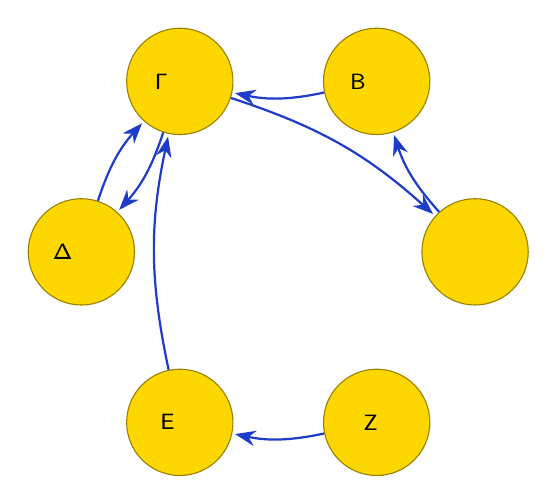
\begin{tikzpicture}
    \foreach \v/\name in {0/Άννα, 1/Βασίλης, 2/Γιώργος, 3/Δήμητρα, 4/Ελένη, 5/Ζωή}
      \node[vertex] (\v) at ({60*\v}:2.5cm) {\name};
    \foreach \u/\v in {0/1, 1/2, 2/0, 2/3, 3/2, 4/2, 5/4}
      \draw[arc] (\u) to (\v);
  \end{tikzpicture}
  \caption{Το γράφημα «ακολουθεί» του \prog{2\_κατευθυνόμενα\_γραφήματα.py}.}
  \label{fig:directed}
\end{figure}

\subsection{Δύο λίστες γειτνίασης}
Σε κατευθυνόμενο γράφημα κάθε κορυφή έχει δύο ειδών γείτονες, άρα κρατάμε δύο λίστες γειτνίασης:
\begin{itemize}
  \item \code{out[v]}: ποιους ακολουθεί ο \code{v} (τα βέλη που \textbf{φεύγουν} από τη \code{v}),
  \item \code{inn[v]}: ποιοι ακολουθούν τον \code{v} (τα βέλη που \textbf{φτάνουν} στη \code{v}).
\end{itemize}

\begin{Piton}
out = [[] for i in range(n)]
inn = [[] for i in range(n)]      # ('in' είναι λέξη-κλειδί της Python, γι' αυτό 'inn')
for u, v in edges:
    out[u].append(v)              # ΜΟΝΟ προς τη μία μεριά: u -> v
    inn[v].append(u)
\end{Piton}

Η διαφορά από το μη κατευθυνόμενο γράφημα είναι μία γραμμή: αντί για \code{adj[v].append(u)}
έχουμε \code{inn[v].append(u)}, δηλαδή η \code{u} μπαίνει σε \textbf{άλλη} λίστα. Αν χρειαζόμαστε
μόνο το «ποιους ακολουθεί ο \code{v}», αρκεί η \code{out}.

\subsection{Ερωτήσεις πάνω στο γράφημα}
\begin{itemize}
  \item \textbf{Βαθμοί:} \code{out\_deg = [len(out[v]) for v in range(n)]} (πόσους ακολουθεί) και
        \code{in\_deg = [len(inn[v]) for v in range(n)]} (πόσοι τον ακολουθούν).
  \item $\sum_v \text{έξω-βαθμός}(v) = \sum_v \text{έσω-βαθμός}(v) = |E|$, γιατί κάθε βέλος έχει μία
        ουρά και μία μύτη. Συγκρίνετε με το $2|E|$ του λήμματος της χειραψίας.
  \item \textbf{Ο πιο δημοφιλής:} αυτός με τον μεγαλύτερο έσω-βαθμό,
        \code{names[in\_deg.index(max(in\_deg))]}.
  \item \textbf{Η σειρά μετράει:} το \code{1 in out[0]} είναι \code{True} (η Άννα ακολουθεί τον
        Βασίλη), ενώ το \code{0 in out[1]} είναι \code{False}.
\end{itemize}

\textbf{Αμοιβαίες ακμές.} Η ακμή \code{[u, v]} είναι αμοιβαία αν υπάρχει και η \code{[v, u]}, δηλαδή
αν \code{u in out[v]}:
\begin{Piton}
mutual = [[u, v] for u, v in edges if u < v and u in out[v]]
\end{Piton}
Χωρίς τη συνθήκη \code{u < v} θα βρίσκαμε κάθε αμοιβαίο ζεύγος δύο φορές, μία ως \code{[2, 3]} και
μία ως \code{[3, 2]}.

\begin{output}
Κορυφές: 6   Ακμές: 7

0 Άννα     ακολουθεί -> ['Βασίλης']
1 Βασίλης  ακολουθεί -> ['Γιώργος']
2 Γιώργος  ακολουθεί -> ['Άννα', 'Δήμητρα']
3 Δήμητρα  ακολουθεί -> ['Γιώργος']
4 Ελένη    ακολουθεί -> ['Γιώργος']
5 Ζωή      ακολουθεί -> ['Ελένη']

0 Άννα     τον/την ακολουθούν <- ['Γιώργος']
1 Βασίλης  τον/την ακολουθούν <- ['Άννα']
2 Γιώργος  τον/την ακολουθούν <- ['Βασίλης', 'Δήμητρα', 'Ελένη']
3 Δήμητρα  τον/την ακολουθούν <- ['Γιώργος']
4 Ελένη    τον/την ακολουθούν <- ['Ζωή']
5 Ζωή      τον/την ακολουθούν <- []

Έξω-βαθμοί: [1, 1, 2, 1, 1, 1]
Έσω-βαθμοί: [1, 1, 3, 1, 1, 0]
Άθροισμα έξω-βαθμών = 7 = άθροισμα έσω-βαθμών = 7 = πλήθος ακμών = 7
Ο πιο "δημοφιλής": Γιώργος με 3 ακόλουθους
Ο 0 ακολουθεί τον 1; True
Ο 1 ακολουθεί τον 0; False
Αμοιβαία ακολουθούνται: [['Γιώργος', 'Δήμητρα']]
\end{output}

\subsection{Σχέδιο με βέλη}
Η \code{draw} είναι ίδια με του προγράμματος 1, εκτός από τις ακμές. Αντί για \code{plt.plot}
χρησιμοποιεί την \code{plt.annotate}, που σχεδιάζει ένα βέλος:
\begin{Piton}
plt.annotate('', xy=(px[v], py[v]), xytext=(px[u], py[u]),
             arrowprops=dict(arrowstyle='-|>', color='b', shrinkA=14, shrinkB=14,
                             mutation_scale=20, connectionstyle='arc3,rad=0.15'))
\end{Piton}
\begin{itemize}
  \item Το βέλος πηγαίνει από το \code{xytext} (η \code{u}) στο \code{xy} (η \code{v}). Το πρώτο
        όρισμα είναι το κείμενο της επισήμανσης: εδώ είναι κενό, θέλουμε μόνο το βέλος.
  \item \code{arrowstyle='-|>'}: βέλος με γεμάτη μύτη. Το \code{mutation\_scale} ορίζει το μέγεθος
        της μύτης.
  \item \code{shrinkA}, \code{shrinkB}: το βέλος ξεκινά και σταματά λίγο πριν από τα κέντρα των
        κορυφών, ώστε η μύτη να φαίνεται έξω από τον κίτρινο κύκλο.
  \item \code{connectionstyle='arc3,rad=0.15'}: το βέλος καμπυλώνει λίγο, ώστε τα $2 \to 3$ και
        $3 \to 2$ να μην πέφτουν το ένα πάνω στο άλλο.
\end{itemize}

\subsection{Σύνοψη}
\begin{center}
\begin{tabularx}{\linewidth}{@{}l Y Y@{}}
\toprule
& \textbf{Μη κατευθυνόμενο} & \textbf{Κατευθυνόμενο} \\
\midrule
ακμή & \code{[u, v]} ίδια με \code{[v, u]} & \code{[u, v]} διαφορετική από \code{[v, u]} \\
λίστες γειτνίασης & \code{adj}: η ακμή μπαίνει στις λίστες και των δύο άκρων & \code{out} και
  \code{inn}: η ακμή μπαίνει στην \code{out[u]} και στην \code{inn[v]} \\
βαθμοί & \code{deg} & \code{out\_deg}, \code{in\_deg} \\
άθροισμα βαθμών & $2|E|$ & $|E|$ (για καθένα από τα δύο) \\
σχέδιο ακμής & \code{plt.plot}: γραμμή & \code{plt.annotate}: βέλος \\
\bottomrule
\end{tabularx}
\end{center}

% =========================================================================
\section{Το αντίστροφο γράφημα}
\noindent Πρόγραμμα: \prog{3\_αντίστροφο\_γράφημα.py}. Το \textbf{αντίστροφο} ενός κατευθυνόμενου
γραφήματος έχει τις ίδιες κορυφές και τα ίδια βέλη, αλλά ανάποδα: για κάθε βέλος $u \to v$ του
αρχικού έχει το βέλος $v \to u$. Για παράδειγμα, το αντίστροφο του γραφήματος «ακολουθεί» είναι το
γράφημα «ακολουθείται από». Οι λίστες γειτνίασης του αντίστροφου είναι ακριβώς η \code{inn} του
προγράμματος 2.

Αυτό το πρόγραμμα είναι οργανωμένο σε \textbf{συναρτήσεις} και αποθηκεύει το γράφημα μόνο με τις
λίστες γειτνίασης \code{adj} (χωρίς λίστα ακμών και χωρίς ονόματα): \code{adj[u]} είναι η λίστα με
τις κορυφές \code{v} για τις οποίες υπάρχει βέλος $u \to v$.

\subsection{Ένα τυχαίο γράφημα}
\begin{Piton}
def random_graph(n, prob):
    adj = [[] for i in range(n)]
    for u in range(n):
        for v in range(n):
            if u != v and random.random() < prob:
                adj[u].append(v)
    return adj
\end{Piton}

Η \code{random.random()} επιστρέφει έναν τυχαίο αριθμό στο $[0, 1)$, οπότε η συνθήκη
\code{random.random() < prob} ισχύει με πιθανότητα \code{prob}. Υπάρχουν $n(n-1)$ πιθανά βέλη (η
συνθήκη \code{u != v} αποκλείει τα βέλη από μια κορυφή στον εαυτό της), άρα κατά μέσο όρο το γράφημα
έχει $\text{prob} \cdot n(n-1)$ ακμές. Για $n = 7$ και $\text{prob} = 0{,}2$ αυτό κάνει $8{,}4$.

\subsection{Η συνάρτηση \code{reverse}}
\begin{Piton}
def reverse(adj):
    n = len(adj)
    rev = [[] for i in range(n)]
    for u in range(n):
        for v in adj[u]:          # βέλος u -> v στο αρχικό ...
            rev[v].append(u)      # ... γίνεται βέλος v -> u στο αντίστροφο
    return rev
\end{Piton}

Το διπλό \code{for} περνά από κάθε βέλος $u \to v$ του γραφήματος \textbf{ακριβώς μία φορά}. Είναι ο
τρόπος να διασχίσουμε όλες τις ακμές όταν έχουμε μόνο λίστες γειτνίασης, και τον ξαναβρίσκουμε στη
\code{draw} του ίδιου προγράμματος. Η \code{reverse} δεν αλλάζει το \code{adj}: φτιάχνει και
επιστρέφει μια \textbf{νέα} λίστα.

\subsection{Έλεγχος: δύο αντιστροφές}
Αν αντιστρέψουμε δύο φορές, πρέπει να πάρουμε πίσω το αρχικό γράφημα:
\begin{Piton}
print('reverse(reverse(g)) == g ;',
      [sorted(a) for a in reverse(r)] == [sorted(a) for a in g])
\end{Piton}

Γιατί \code{sorted}; Η σειρά των γειτόνων μέσα σε μια λίστα γειτνίασης δεν έχει σημασία για το
γράφημα, αλλά έχει σημασία για τη σύγκριση \code{==} λιστών. Για παράδειγμα, για
\code{adj = [[2, 1], [], []]} η \code{reverse(reverse(adj))} δίνει \code{[[1, 2], [], []]}: το ίδιο
γράφημα, διαφορετική λίστα. Ταξινομώντας κάθε λίστα συγκρίνουμε τα γραφήματα και όχι τη σειρά.

\subsection{Μια εκτέλεση}
Το γράφημα είναι τυχαίο, άρα κάθε εκτέλεση δίνει άλλο αποτέλεσμα. Μια εκτέλεση έδωσε
(Σχήμα~\ref{fig:reverse}):

\begin{output}
Αρχικό γράφημα:
   0 -> [4, 5]
   1 -> [4]
   2 -> [0, 4]
   3 -> [4]
   4 -> []
   5 -> [0]
   6 -> [1, 5]

Αντίστροφο γράφημα:
   0 -> [2, 5]
   1 -> [6]
   2 -> []
   3 -> []
   4 -> [0, 1, 2, 3]
   5 -> [0, 6]
   6 -> []

reverse(reverse(g)) == g ; True
\end{output}

\begin{figure}[h]
  \centering
  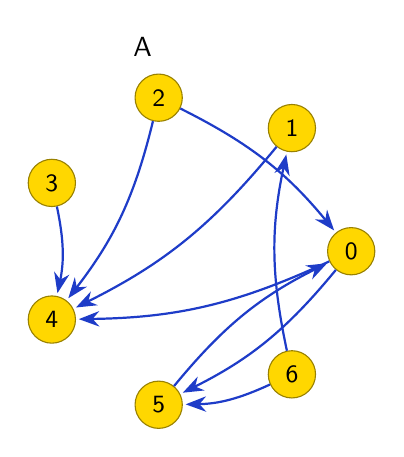
\begin{tikzpicture}
    \node at (0, 2.6) {\sffamily Αρχικό γράφημα};
    \foreach \v in {0,...,6}
      \node[small vertex] (\v) at ({360/7*\v}:2cm) {\v};
    \foreach \u/\v in {0/4, 0/5, 1/4, 2/0, 2/4, 3/4, 5/0, 6/1, 6/5}
      \draw[arc] (\u) to (\v);
  \end{tikzpicture}
  \hspace{1.2cm}
  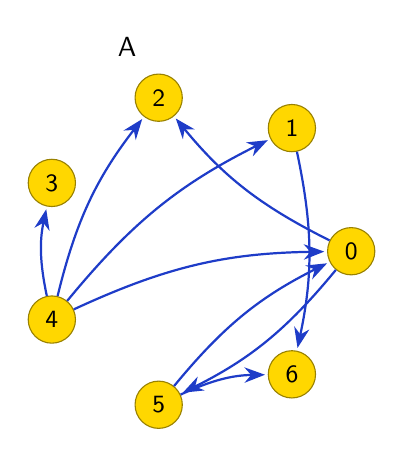
\begin{tikzpicture}
    \node at (0, 2.6) {\sffamily Αντίστροφο γράφημα};
    \foreach \v in {0,...,6}
      \node[small vertex] (\v) at ({360/7*\v}:2cm) {\v};
    \foreach \u/\v in {0/2, 0/5, 1/6, 4/0, 4/1, 4/2, 4/3, 5/0, 5/6}
      \draw[arc] (\u) to (\v);
  \end{tikzpicture}
  \caption{Ένα τυχαίο γράφημα ($n = 7$, $\text{prob} = 0{,}2$) και το αντίστροφό του.}
  \label{fig:reverse}
\end{figure}

Παρατηρήστε:
\begin{itemize}
  \item Ο \textbf{έξω-βαθμός} κάθε κορυφής στο αρχικό είναι ο \textbf{έσω-βαθμός} της στο
        αντίστροφο, και αντίστροφα.
  \item Στην κορυφή 4 φτάνουν τέσσερα βέλη αλλά δεν φεύγει κανένα. Στο αντίστροφο φεύγουν από αυτήν
        τέσσερα βέλη και δεν φτάνει κανένα.
  \item Το αμοιβαίο ζεύγος $0 \leftrightarrow 5$ μένει ίδιο: το αντίστροφο του $0 \to 5$ είναι το
        $5 \to 0$, που υπήρχε ήδη, και αντίστροφα.
\end{itemize}

\subsection{Δύο σχήματα δίπλα-δίπλα}
Εδώ η \code{draw(adj, title)} παίρνει τις λίστες γειτνίασης και διασχίζει τις ακμές με το ίδιο διπλό
\code{for} όπως η \code{reverse}. Δεν καλεί την \code{plt.show()}, ώστε να ζωγραφίσουμε πρώτα και τα
δύο γραφήματα:
\begin{Piton}
plt.subplot(1, 2, 1)       # 1 γραμμή, 2 στήλες, 1ο σχήμα
draw(g, 'Αρχικό γράφημα')
plt.subplot(1, 2, 2)       # 2ο σχήμα
draw(r, 'Αντίστροφο γράφημα')
plt.show()
\end{Piton}
Η \code{plt.subplot(1, 2, k)} χωρίζει το παράθυρο σε 1 γραμμή και 2 στήλες και διαλέγει το
\code{k}-οστό κομμάτι. Ό,τι ζωγραφίσουμε μετά πηγαίνει σε αυτό το κομμάτι. Η \code{plt.title} βάζει
τίτλο σε κάθε κομμάτι.

% =========================================================================
\section{Ασκήσεις}

\begin{enumerate}
  \item Γράψτε τη συνάρτηση \code{edges\_from\_adj(adj)} που επιστρέφει τη λίστα ακμών ενός μη
        κατευθυνόμενου γραφήματος, \textbf{χωρίς διπλότυπα}. (Υπόδειξη: κρατήστε μόνο τα
        \code{[u, v]} με \code{u < v}.) Ελέγξτε ότι για το \code{adj} του προγράμματος 1 δίνει
        πίσω τις 7 ακμές.
  \item Φτιάξτε τη λίστα ακμών του \textbf{κύκλου} $C_n$ (η $i$ συνδέεται με την $(i+1) \bmod n$)
        και του \textbf{πλήρους γραφήματος} $K_n$ (όλα τα ζεύγη). Ζωγραφίστε τα με τη \code{draw} του
        προγράμματος 1. Πόσες ακμές έχει το $K_n$; Ελέγξτε το λήμμα της χειραψίας.
  \item Στο πρόγραμμα 1, τυπώστε \textbf{όλους} τους «πιο κοινωνικούς», όχι μόνο τον πρώτο.
  \item Στο πρόγραμμα 1, γράψτε τη συνάρτηση \code{friends\_of\_friends(adj, v)} που επιστρέφει τους
        φίλους των φίλων της \code{v} που \textbf{δεν} είναι ήδη φίλοι της (ούτε η ίδια η \code{v}),
        χωρίς διπλότυπα. Είναι οι «προτάσεις φιλίας» ενός κοινωνικού δικτύου.
  \item Στο πρόγραμμα 2, βρείτε ποιοι δεν ακολουθούνται από κανέναν (έσω-βαθμός 0) και ποιοι δεν
        ακολουθούν κανέναν (έξω-βαθμός 0). Για κάθε \code{v}, τυπώστε όσους ακολουθεί η \code{v}
        χωρίς να την ακολουθούν πίσω.
  \item Χρησιμοποιήστε την \code{reverse} του προγράμματος 3 για να ελέγξετε ότι
        \code{reverse(out)} δίνει την \code{inn} του προγράμματος 2.
  \item Ένα κατευθυνόμενο γράφημα είναι \textbf{συμμετρικό} αν για κάθε βέλος $u \to v$ υπάρχει και
        το $v \to u$. Γράψτε τη συνάρτηση \code{is\_symmetric(adj)}. (Υπόδειξη: ένα γράφημα είναι
        συμμετρικό ακριβώς όταν είναι ίσο με το αντίστροφό του.)
  \item Τρέξτε τη \code{random\_graph(7, 0.2)} 10000 φορές και υπολογίστε τον μέσο όρο του πλήθους
        των ακμών. Συμφωνεί με το $\text{prob} \cdot n(n-1) = 8{,}4$;
\end{enumerate}

% =========================================================================
\newpage
\appendix
\PitonOptions{line-numbers}
\section{Τα προγράμματα της διάλεξης}

\subsection{\prog{1\_μη\_κατευθυνόμενα\_γραφήματα.py}}
\pyfile{1_μη_κατευθυνόμενα_γραφήματα.py}

\subsection{\prog{2\_κατευθυνόμενα\_γραφήματα.py}}
\pyfile{2_κατευθυνόμενα_γραφήματα.py}

\subsection{\prog{3\_αντίστροφο\_γράφημα.py}}
\pyfile{3_αντίστροφο_γράφημα.py}

\end{document}
